\section{Einleitung}
Der Klimawandel äussert sich in der Schweiz überdurchschnittlich. So ist die mittlere Jahrestemperatur in der Schweiz seit Messbeginn im Jahr 1864 um 2 °C gestiegen, was rund doppelt so stark ist, wie das globale Mittel. In der Schweiz wird rund ein Drittel aller Treibhausgasemissionen durch den Verkehr (ohne internationalen Flug- und Schiffsverkehr) verursacht \cite{BAFU}. Um das \emph{Netto-Null-Ziel} der \emph{Langfristigen Klimastrategie der Schweiz} zu erfüllen, müssen daher unteranderem im Verkehrssektor Veränderungen vorgenommen und Entwicklungen getätigt werden.\\
Louis Palmer, ein Schweizer Umweltaktivist und "\emph{Macher}", umrundete im Jahr 2004 als erster mit einem Elektrofahrzeug - dem Solarfahrzeug \emph{Solartaxi} - die Erde und gilt somit als ein Pionier im Bereich der Elektromobilität \cite{Palmer}.\\
Sein neustes Projekt ist der \emph{Solar Butterfly} - ein autarker Wohnwagen, mit welchem er "eine Reise zu den Klimalösungen dieser Welt [...] im ersten solarbetriebenen <<Mobile Home>> der Welt" antreten will. Ein Ziel von Palmer ist es, mit dem Solar Butterfly weltweite Aufmerksamkeit zu erregen und so nachhaltige Lösungen im Bereich des Klimaschutzes und Elektromobilität zu ermutigen und voranzutreiben.\\
Die erneute Weltumrundung soll dieses Mal "mit etwas mehr Komfort" geschehen. Seine Vision ist es, ein Wohnwagen, mit zwei Ausziehbaren Wohnelementen und rund 100 $m^2$ integrierte Photovoltaikfläche, zu realisieren. Der Wohnwagen soll sich selbst mit Solar-Energie versorgen und autonom operiert werden können. Im Rahmen dieser Bachelorarbeit soll, in Zusammenarbeit mit drei weiteren Studenten der HSLU T\&A, seine Vision des Solar Butterflys in die Realität umgesetzt werden.\\
Das Projekt wurde neben dieser Arbeit in die weiteren Teilgebiete \emph{Auslegung Klappmechanismen}, \emph{Auslegung Antriebstechnik} und \emph{Auslegung Solar Butterfly (Globales CAD)} aufgeteilt.\\
Das Auslegen der Klappmechanismen beinhaltet das Entwerfen und Dimensionieren aller beweglichen Teilen wie die klappbaren Panelen und den Ausfahrmechanismus der seitlichen Raumelementen. Die Arbeit \emph{Auslegen der Antriebstechnik} befasst sich mit der Technik, mit welcher die beweglichen Bauteile in Bewegung gesetzt werden. Im Teilgebiet \emph{Auslegung Solar Butterfly (Globales CAD)} werden die jeweiligen Teilgebiete zusammengeführt. Ebenfalls beinhaltet diese Aufgabenstellung das Erstellen eines globalen CAD-Modells, das Zusammentragen der allgemeinen Anforderungen sowie eine Risikobewertung des Projektes.

\subsection{Aufgabenstellung}
\label{Aufgabenstellung}
Der Fokus dieser Arbeit liegt in der Festlegung der Anforderungen und Auslegungskriterien, der Ausarbeitung eines detaillierten Lastenheftes, sowie in der Dimensionierung der Grundstruktur. Zur Bestimmung von Schnittgrössen, mit welchen Handrechnungen gemacht oder verifiziert werden können, soll dabei ein globales FEM-Modell zur Anwendung kommen. Ebenfalls sollen zulässige Festigkeitswerte abhängig von der gewählten Bauweise abgeschätzt werden (Design-Allowables).\\
Weiter beinhaltet die Aufgabenstellung eine enge Zusammenarbeit mit den drei weiteren Mitstudenten. Es soll sich aktiv an der Lösungsfindung und weiteren Ausarbeitung des Konzeptes beteiligt und dabei besonders die Aspekte und Position der strukturellen Integrität berücksichtigt und vertreten werden.

\subsection{Vorgehen und Methodik}
In diesem Kapitel wird beschrieben, wie beim Lösen der Aufgabenstellung vorgegangen wird. Die Struktur des vorliegenden Dokumentes entspricht dabei dem nun vorgestellten Vorgehen.

In einem ersten Schritt wird definiert, welchen Anforderungen der Solar Butterfly als Ganzes, von einem Standpunkt der strukturellen Integrität aus betrachtet, gerecht werden muss. Weiter werden die Auslegungskriterien bestimmt. Sie beschreiben im Detail, nach welchen Kriterien die einzelnen Komponenten des Solar Butterflys ausgelegt werden. So wird zum Beispiel beschrieben, welche Kriterien die Sandwichplatten erfüllen müssen, dass diese unter Belastung nicht beulen.\\
Anschliessend wird ein Lastenheft erstellt, welches eine Zusammenstellung von verschiedenen Lastfällen darstellt, welchen der Solar Butterfly ausgesetzt werden kann. Ferner werden sogenannte \emph{Modi} eingeführt, welche die Zustände und Positionen, in welchen sich der Solar Butterfly befinden kann, beschreiben. Für die Lastfälle des Lastenheftes - und Kombinationen davon - soll der Solar Butterfly in den verschiedenen Modi ausgelegt werden.\\
Als nächstes wird der Solar Butterfly grob als "Kasten" idealisiert. Es werden für die kritischen Lastfälle Handrechnungen durchgeführt, um so Kräfte und Schubflüsse bestimmen zu können. Dies wird zum einen gemacht, um die Grössenordnung der Lasten besser abschätzen zu können. Andererseits kann dadurch eine erste grobe Dimensionierung der wichtigsten Komponenten erfolgen und die zu diesem Zeitpunkt bereits getroffenen Annahmen bezüglich den Lasten beurteilt werden.\\
In einem letzten Schritt wird der Solar Butterfly in FEM-Berechnungen verschiedenen kritischen Lastfällen ausgesetzt, um so Lastpfade und Schnittkräfte zu bestimmen, anhand welchen eine Verifizierung der Handrechnungen und eine exaktere Dimensionierung und Beurteilung der Komponenten und Verbindungen erfolgen kann. Weiter können mit FEM-Berechnungen für die Funktionstauglichkeit kritische Verformungen festgestellt werden, welche in der weiteren Ausarbeitung des Konzeptes berücksichtigt werden sollen.\\
Im Kapitel \ref{Diskussion} werden zum Schluss die erlangten Erkenntnisse zusammengefasst und Empfehlungen für das weitere Vorgehen abgegeben.

\subsection{Der Solar Butterfly}
Ziel diese Kapitels ist es, einen Überblick des Solar Butterflys zu geben und die Funktionen der wichtigsten Komponenten zu erklären.
In den folgenden drei Abbildungen ist der Solar Butterfly schematisch dargestellt. Im Anhang \ref{Bilder SB} sind realitätsgetreuere Abbildungen des CAD-Modelles und im elektronischen Anhang \ref{Bilder des Solar Butterflys} Detailansichten und weitere Bilder zu finden.

\begin{figure}[H]
  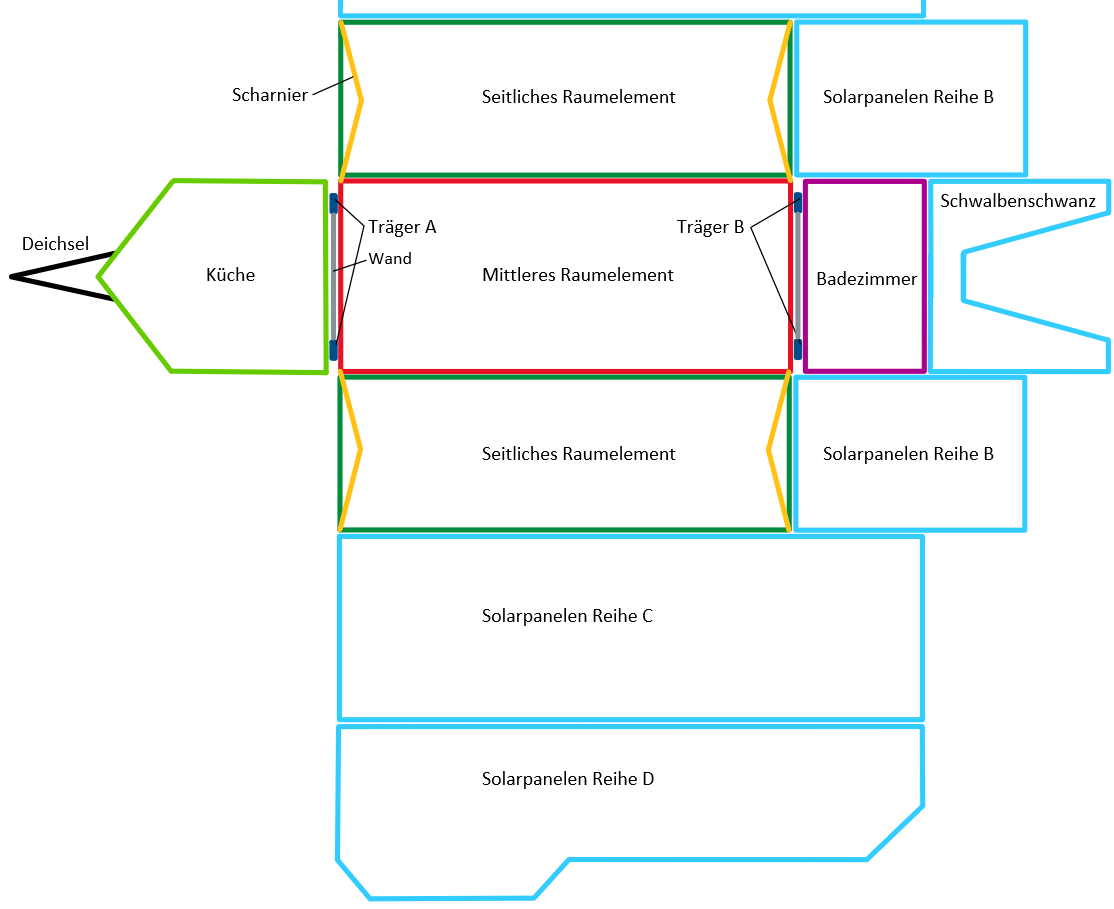
\includegraphics[width=\linewidth]{04_Figures/SB1.png}
  \caption{Der Solar Butterfly von Oben}
  \label{img:SB1}
\end{figure}

\begin{figure}[H]
  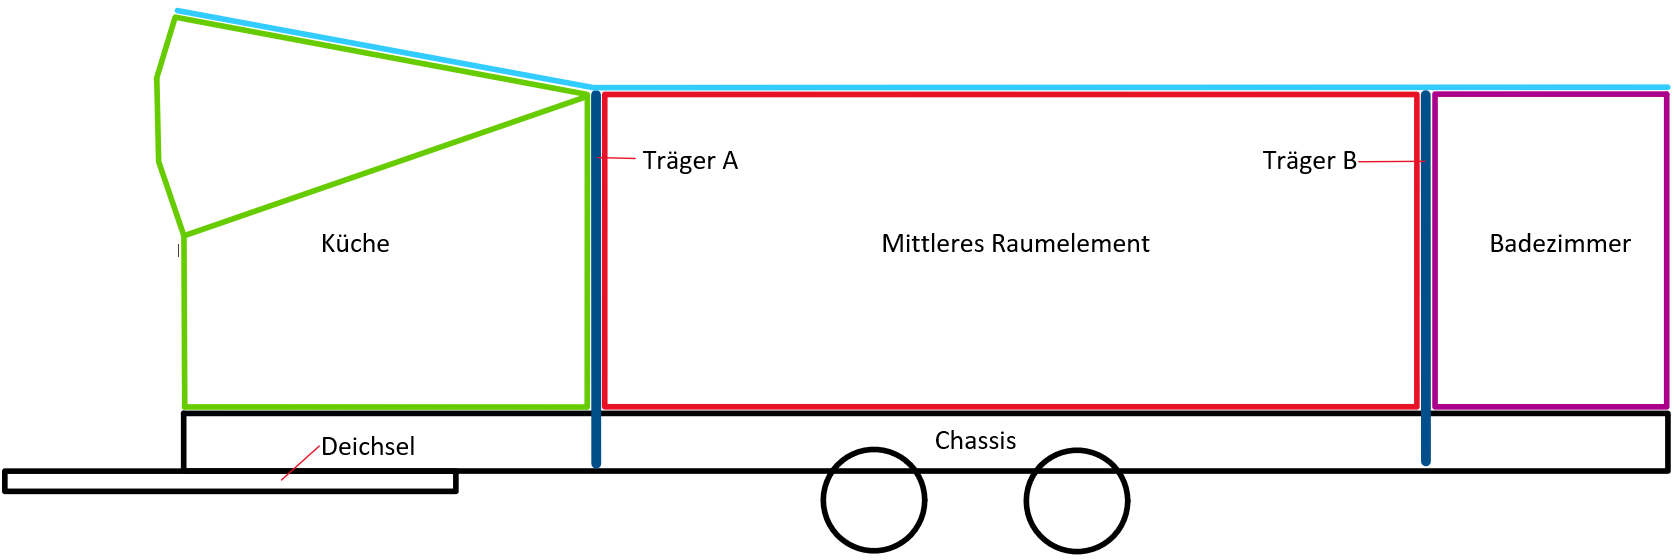
\includegraphics[width=\linewidth]{04_Figures/SB3.png}
  \caption{Seitenansicht des Solar Butterflys}
  \label{img:SB3}
\end{figure}

\begin{figure}[H]
  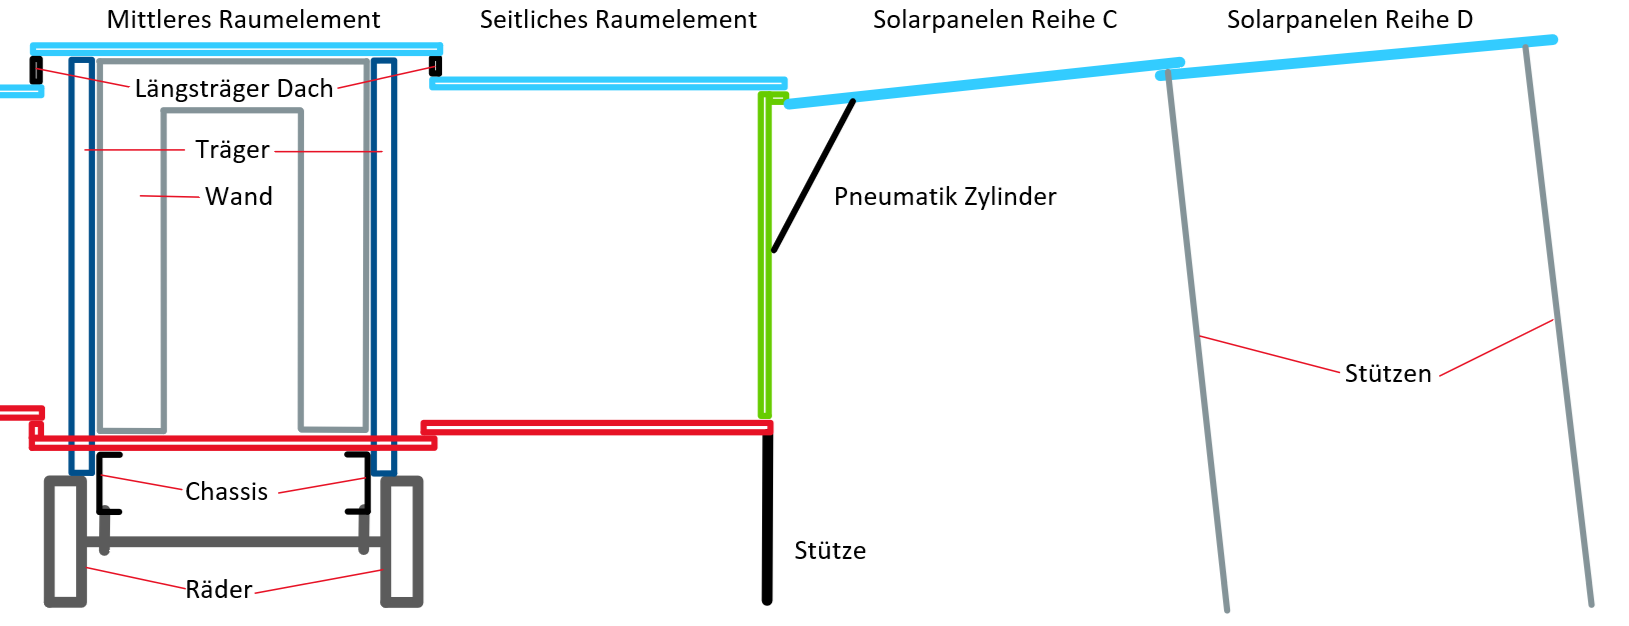
\includegraphics[width=\linewidth]{04_Figures/SB2.png}
  \caption{Schnittansicht des Solar Butterflys}
  \label{img:SB2}
\end{figure}

Grundbaustein des Solar Butterflys ist das Chassis, an welchem die Träger A und B und der Boden befestigt sind. An den Trägern A und B sind wiederrum die Scharniere, an welchen die seitlichen Raumelemente ausgefahren werden können, sowie die Wände und das Dach befestigt.\\
In Bewegung gebracht werden die Bauteile des Solar Butterflys durch Pneumatik. Die seitlichen Raumelemente werden durch je zwei Pneumatikzylinder im Chassis aus- und eingefahren. Die beweglichen Solarpanelen werden ebenfalls mittels Pneumatik, in Kombination mit Gasdruckfedern, bewegt. Die Solarpanelen der Reihe D können über Teleskopscharniere unterhalb der Reihe C hervorgeschoben werden.

Der Solar Butterfly soll verschifft werden können, muss daher in einen Container passen und darf die Masse von 2.64 x 10.2 x 2.3 (Höhe x Länge x Breite) nicht überschreiten. Die Gewichtslimite des Solar Butterflys beträgt für Europa 2200 und für den Rest der Welt 3000 kg und stellt eine der grössten Herausforderungen des Projektes dar. Die Thematik des Gewichtes prägt entsprechend die Arbeiten und hat die getroffenen Entscheidungen massgebend beeinflusst.

Während der Fahrt sollen die beweglichen Teile des Solar Butterflys über formschlüssige Verbindungen mit dem Rest der Struktur verbunden werden. So kann eine sichere Fahrt auch bei hohen Geschwindigkeiten gewährleistet werden.

Im Innern des Solar Butterflys soll sich Moblilar befinden (Sofa, Tische etc.) welches während der Fahrt befestigt und verstaut werden muss.

Bilder sind von Huber
\subsection{Projektorganisation}
Wie in der Einleitung beschrieben, sind drei weitere Maschinenbaustudenten mit Ihrer Bachelorarbeit an dem Projekt Solar Butterfly beteiligt. Jedem der Studenten steht ein Dozent zur Betreuung und Unterstützung zur Verfügung. Mit den insgesamt acht Parteien (mit dem Auftraggeber neun) ist entsprechend viel Austausch und Kommunikation nötig. Es wurden Wöchentliche Meetings, abwechslungsweise über Videokonferenz oder an der HSLU vor Ort, abgehalten. Zusätzlich zu diesen Meetings wurden Wöchentliche Meetings mit dem betreuenden Dozenten Dejan Roman\v{c}uk abgehalten.
\newpage
